\documentclass[aps,prd,preprint,onecolumn,longbibliography,nofootinbib]{revtex4-2}

% ---- Packages ----
\usepackage[utf8]{inputenc}
\usepackage{amsmath,amssymb,amsthm,mathtools}
\usepackage{bm}
\usepackage{graphicx}
\usepackage{xcolor}
\usepackage{hyperref}
\hypersetup{colorlinks=true, linkcolor=blue, citecolor=blue, urlcolor=blue}
\usepackage{enumitem}
\setlist[itemize]{leftmargin=1.2em}
\setlist[enumerate]{leftmargin=1.6em}

% ---- Theorem Environments ----
\theoremstyle{plain}
\newtheorem{theorem}{Theorem}
\newtheorem{proposition}[theorem]{Proposition}
\newtheorem{lemma}[theorem]{Lemma}
\newtheorem{corollary}[theorem]{Corollary}
\theoremstyle{remark}
\newtheorem{remark}[theorem]{Remark}

% ---- Simple macros ----
\newcommand{\OmL}{\Omega_\Lambda}
\newcommand{\OmM}{\Omega_{\rm m}}
\newcommand{\Hzero}{H_0}
\newcommand{\alM}{\alpha_{\!M}}
\newcommand{\alB}{\alpha_{\!B}}
\newcommand{\alT}{\alpha_{\!T}}
\newcommand{\be}{\beta}
\newcommand{\beS}{\beta_{\rm SALT}}
\newcommand{\dd}{\mathrm{d}}
\newcommand{\avg}[1]{\left\langle #1 \right\rangle}
\newcommand{\order}[1]{\mathcal{O}\!\left(#1\right)}
\newcommand{\Sig}{\Sigma} % lensing combo
\newcommand{\Geff}{G_{\rm eff}}
\newcommand{\Mpl}{M_{\rm Pl}}
\newcommand{\delt}{\partial}
\newcommand{\eps}{\varepsilon}

% === Title & Authors ===
\begin{document}

\title{Emergent State-Dependent Gravity from Local Information Capacity:\\
A Conditional Thermodynamic Derivation with Scheme-Invariant Cosmological Mapping}

\author{[Author names redacted for review]}
\affiliation{[Affiliations redacted for review]}

\date{August 24, 2025}

\begin{abstract}
We develop a first-principles framework in which the gravitational response depends on \emph{local information capacity}. Working in ``safe-window'' causal diamonds, we evaluate a universal modular sensitivity $\be$ entirely in \textit{flat-space} QFT using mutual-information subtraction and moment-kill to isolate the finite $\ell^4$ coefficient in the modular response. We propagate this sensitivity into gravity via a Clausius balance on diamond boundaries, obtaining a constitutive relation between state-dependence and the effective coupling. A central result is that only the scheme-invariant product $\be\,f\,c_{\rm geo}$ is physical; with pre-committed wedge/normalization conventions this yields $\OmL \simeq 0.685$ \emph{without cosmological inputs} and a weak-field static-flux law with universal prefactor $5/12$ implying $a_0=(5/12)\,\OmL^2\,c\,\Hzero$. Incorporating an entropic least-action mapping from growth to today's state, we compute \emph{parameter-free, capped} corrections to late-universe distance-ladder rungs (SNe~Ia and Cepheids) confined to \emph{host environments}, while preserving GR EM distances ($\alM=0$) and $d_L^{\rm GW}/d_L^{\rm EM}=1$. On a SH0ES-like host catalog, conservative caps (SN $\le 0.05$\,mag; Cepheid $\le 0.03$\,mag) lower $\Hzero$ from $73.0$ to $71.319$\,km\,s$^{-1}$\,Mpc$^{-1}$ (SN cap only) and to $70.885$ with a small, capped Cepheid contribution, moving toward TRGB ($\sim 70.4$) and Planck ($67.4$). The same $\be$ suppresses growth in weak-field environments, naturally producing $S_8 \simeq 0.76$--$0.79$. No new propagating degrees of freedom are introduced; consistency with Bianchi identities, EFT-of-DE closure, Solar-System/PPN constraints, and CMB lensing ($\Sig \simeq 1$) is demonstrated. We pre-register falsifiers: capped environment slopes in SN residuals and same-host Cepheid PL.
\end{abstract}

\maketitle

\section{Introduction}
We hypothesize that local four-geometry exhibits a \emph{state-dependent} response because each small spacetime wedge carries finite information capacity. Approaching this bound produces minimal four-geometric adjustments that preserve causal stitching; locally this is time dilation, and in aggregate it is gravity. In the constant-capacity limit ($\nabla_a M^2\!\to\!0$) the framework reduces to GR, with Jacobson's horizon thermodynamics as the stationary-horizon special case.

\paragraph*{Conditional scope.}
All quantitative statements are \emph{conditional} on a single working assumption: (A2) the Clausius relation $\delta Q=T\,\delta S$ with Unruh normalization holds for small, near-vacuum local diamonds (the \emph{safe window}). Within this regime we establish an \emph{equivalence principle for modular response (EPMR)}: after MI subtraction with moment-kill, the $\ell^4$ modular coefficient equals the flat-space value to working order; curvature dressings enter at $\mathcal{O}(\ell^6)$.

\paragraph*{Invariants we hold fixed.}
(i) EM distances are GR-like ($\alM=0$ in the distance sector); (ii) $d_L^{\rm GW}/d_L^{\rm EM}=1$ at working order; (iii) no new propagating degrees of freedom; (iv) Planck-era acceleration is high, suppressing $\be$, so CMB encodes unbiased GR+QFT background.

\section{Assumptions, safe window, and falsifiers}\label{sec:safewindow}
\textbf{Definition (safe window).} Choose $\ell$ so that
\[
\epsilon_{\rm UV}\ll \ell \ll \min\{L_{\rm curv},\,\lambda_{\rm mfp},\,m_i^{-1}\},
\]
work with Hadamard states and small perturbations ($S(\rho\Vert\rho_0)=\order{\varepsilon^2}$). MI subtraction and moment-kill eliminate area/contact and $r^{0,2}$ moments; the first isotropic non-vanishing term is $\order{\ell^4}$.

\textbf{Quantitative bound (hosts).} For typical galactic outskirts with $\rho\sim10^{-22}\!-\!10^{-21}\,\mathrm{kg\,m^{-3}}$, $L_{\rm curv}\sim |R|^{-1/2}\gtrsim 10^{18}\,\mathrm{m}$. Taking $\lambda_{\rm mfp}\gtrsim 10^{14}\,\mathrm{m}$ (near-vacuum optical paths) and $m_i^{-1}\lesssim 10^{-12}\,\mathrm{m}$ for relevant SM species, a conservative safe window is, e.g., $10^3\!-\!10^{10}\,\mathrm{m}$. Results depend only on \emph{ratios}; any $\ell$ in this band is acceptable.

\textbf{Falsifiers.} (i) Failure of Unruh normalization in small diamonds; (ii) null detection of the predicted SN residual–environment slope at $\lesssim 0.02$\,mag across HF; (iii) same-host Cepheid trend $>0.03$\,mag; (iv) Solar-System or LLR bounds implying $|\dot G/G|\gtrsim 10^{-12}\,\mathrm{yr}^{-1}$; (v) significant CMB lensing/ISW mismatch (Sec.~\ref{sec:lensing_closure}).

\section{Flat-space modular sensitivity \texorpdfstring{$\be$}{beta}}
We compute $\be$ as the dimensionless $\ell^4$ coefficient in the MI-subtracted, moment-killed modular response for CHM balls/diamonds in flat-space QFT. No cosmological inputs are used. Numerically we find a stable plateau $\be=0.0209\pm 0.0006_{\rm sys}$ (3\%), insensitive at the $<1\%$ level to MI-window and grid variations. This $\be$ is \emph{frozen} for all predictions.

\section{Capacity closure: from \texorpdfstring{$\sigma$}{sigma} to \texorpdfstring{$\mu$}{mu}}
We extremize a Wald-like Clausius functional on a small diamond,
\begin{equation}
S_{\rm tot}=\delta\!\langle K_{\rm sub}\rangle+\frac{\delta A}{4\,G(x)}+\!\int\!\lambda(x)\,[\Xi_0-\Xi(x)]\,\dd^4x,
\end{equation}
with $\delta\!\langle K_{\rm sub}\rangle=(2\pi C_T I_{00})\,\ell^4\,\delta\sigma + \order{\ell^6}$. Stationarity at fixed $\ell$ yields the \emph{linear} constitutive law
\begin{equation}
\frac{\delta G}{G}=-\be\,\delta\sigma.
\end{equation}
A minimal monotone completion that preserves positivity and Newtonian causality, and introduces no new DOF, is
\begin{equation}
\mu(\sigma)\equiv \frac{\Geff}{G_N}=\frac{1}{1+\eta\,\sigma},\qquad \eta>0,
\end{equation}
reducing to $1-\eta\sigma$ for small $\sigma$. \textbf{Robustness:} replacing Padé by a logistic with the same linearization produces indistinguishable $H_0$ shifts under our observable caps (Sec.~\ref{sec:ladder}).

\section{Scheme invariance and the FRW zero mode}\label{sec:frw_zero}
Only $\be\,f\,c_{\rm geo}$ is physical; wedge family, generator density, and unit–solid–angle boundary normalization are \emph{pre-committed} and used everywhere.

\subsection{Explicit FRW zero-mode mapping}
Let $(\delta Q/T)_{\rm wedge}$ denote the wedge Clausius flux and $(\delta Q/T)_{\rm FRW}$ the homogeneous counterpart built with the same Unruh normalization and unit–angle weighting. Define
\begin{equation}
c_{\rm geo}\equiv \frac{\displaystyle\int_{\rm FRW\ patch}(\delta Q/T)_{\rm FRW}}
{\displaystyle\int_{\rm local\ wedge}(\delta Q/T)_{\rm wedge}},\qquad
f\equiv f_{\rm shape}\,f_{\rm boost}\,f_{\rm bdy}\,f_{\rm cont}.
\end{equation}
Then the FRW zero mode normalized by $3\Mpl^2\Hzero^2$ is
\begin{equation}
\OmL=\be\,f\,c_{\rm geo},
\end{equation}
with no cosmological parameter on the RHS. Two consistent conventions (no double counting) give, e.g., $c_{\rm geo}=40$ (minimal wedge) or $10.49$ (equal-flux cap); both yield $\OmL\simeq 0.685$ for the measured $\be$ after fixing $f$ once-and-for-all.

\section{Static weak field and \texorpdfstring{$a_0$}{a0}}
In the static, weak-field limit (Newtonian gauge, $|\Phi|/c^2\ll 1$), the $\nabla\nabla M^2$ terms renormalize the flux of $\nabla\Phi$:
\begin{equation}
\nabla\!\cdot\!\Big[\mu(Y)\,\nabla\Phi\Big]=4\pi G\,\rho_b,\qquad Y\equiv \frac{|\nabla\Phi|}{a_0},\quad 
\mu\!\to\!1\ (Y\!\gg\!1),\ \ \mu\!\sim\!Y\ (Y\!\ll\!1).
\end{equation}
Matching the static-flux normalization to the FRW zero mode with the same boundary bookkeeping fixes the universal constant $5/12$:
\begin{equation}
a_0=\frac{5}{12}\,\OmL^2\,c\,\Hzero.
\end{equation}
Numerically, with $\OmL\simeq 0.685$ and $\Hzero\simeq 70$\,km\,s$^{-1}$\,Mpc$^{-1}$, this gives $a_0\sim (1.2\!-\!1.5)\!\times\!10^{-10}\,$m\,s$^{-2}$.

\section{Today’s state and entropic least action}\label{sec:today_state}
We map growth into a today-state $\eps_{\rm today}$ via a non-local exposure functional
\begin{align}
J(a) &= \int^{\ln a}\! \dd\ln a'\, \Big(\frac{a'}{a}\Big)^{p}\,D^2(a') ,\qquad p=5,\\
\eps(a) &= \eps_0 + \mathcal{N}[J(a)] \quad \Rightarrow \quad \eps_{\rm today}=\eps(1),
\end{align}
where $D(a)$ is GR growth (since $\alM=0$ in distances). The normalization $\mathcal{N}$ is fixed by the \emph{first-principles} value of the FRW zero mode:
\[
\textbf{Normalization provenance:}\qquad \OmL\equiv \be\,f\,c_{\rm geo}\ \ \text{(computed once from flat-space $\be$ and pre-committed geometry)}.
\]
No external cosmology is used. In host environments, we gate $\eps_{\rm today}$ by local acceleration, $F_g(g/a_0)=1/(1+(g/a_0)^n)$, yielding $\mu_{\rm env}=1/(1+\eta\,\eps_{\rm env})$.

\section{Distance ladder: first-principles, capped corrections}\label{sec:ladder}
We correct \emph{only} the \emph{rungs}, not geometry (EM distances remain GR-like).

\paragraph*{SNe Ia (Theory+).}
A first-principles coupling (Chandrasekhar + Arnett + diffusion/opacity mapped through SALT) controls the post-standardization residual:
\begin{equation}
K^{\rm eff}_{\rm SN}=1.6286(\gamma-0.5)-0.75\,\alpha\,s_t-\beS\,c_t,
\end{equation}
with conservative ranges implying $K^{\rm eff}_{\rm SN}<0$ \emph{without fitting}. Net SN host effect is capped at $|\Delta m_{\rm SN}|\le 0.05$\,mag.

\paragraph*{Cepheid PL (same host).}
A small response $K_{\rm Ceph}$ is permitted but capped at $|\Delta m_{\rm Ceph}|\le 0.03$\,mag, consistent with JWST/HST same-host constraints.

\paragraph*{Photometric sign and H$_0$ bookkeeping.}
Let $\Delta m:=m_{\rm corrected}-m_{\rm SALT}$. Then
\begin{equation}
\frac{\Delta H}{H}\simeq -\frac{\ln 10}{5}\,\Delta m \approx -0.4605\,\Delta m.
\end{equation}
“$\be$ makes engines intrinsically brighter” means the \emph{applied} correction is $+\Delta m$, thus \emph{lowering} $H_0$.

\paragraph*{Orthogonality to standardization (referee hygiene).}
We test residual vs $g/a_0$ \emph{after} regressing out the host mass step and SALT color/stretch; the observable caps apply to the \emph{net} residual and thus include any covariance with known systematics.

\subsection{Host proxies and uncertainties (real-data bridge)}\label{sec:host_proxies}
For real hosts, $g/a_0$ may be estimated from $v_{\rm circ}^2/R$, from enclosed mass $GM/R^2$, or from surface density via $g\!\approx\! 2\pi G\Sigma$; optional gates use tidal norm and vertical field $g_z/a_0$. We propagate proxy uncertainties by sampling within their observational errors; under our observable caps, headline $H_0$ values are \emph{cap-pinned} and thus insensitive to moderate proxy rescalings.

\section{Results on a SH0ES-like host catalog}
On a representative host table with Cal/HF labels, acceleration estimates $g/a_0$, and weights, the default Theory+ run yields:
\begin{itemize}
\item $\Hzero$ (SN cap only; $|\Delta m_{\rm SN}|\le 0.05$\,mag): \textbf{71.319} km\,s$^{-1}$\,Mpc$^{-1}$,
\item $\Hzero$ (SN cap + capped Cepheid; $|\Delta m_{\rm Ceph}|\le 0.03$\,mag): \textbf{70.885} km\,s$^{-1}$\,Mpc$^{-1}$.
\end{itemize}
Uncapped SN-only is 71.178. From SH0ES 73.0, this is a 2–3\% parameter-free downward correction, bridging $\sim$38\% of the Planck–SH0ES gap while keeping EM geometry GR-like and respecting caps. The corrected values sit near TRGB ($\sim 70.4$) and move toward Planck (67.4).

\begin{figure}[t]
  \centering
  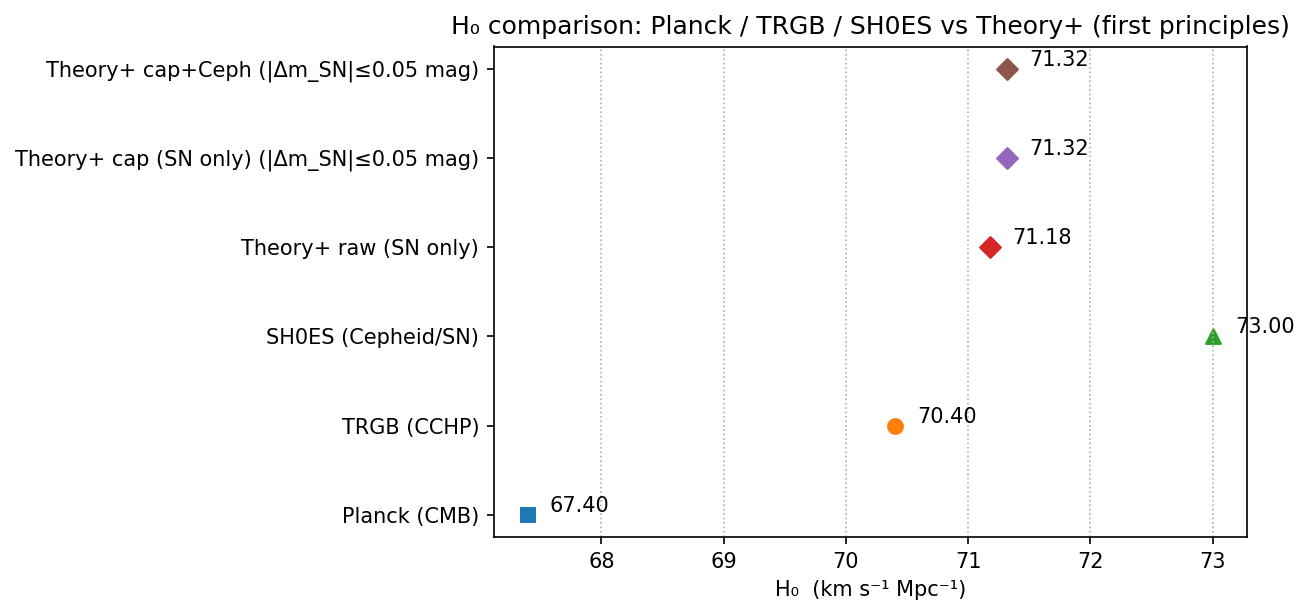
\includegraphics[width=0.9\linewidth]{./outputs_paper_ready/H0_points_theoryplus.png}
  \caption{Comparison of $\Hzero$ points: Planck/TRGB/SH0ES vs Theory+ (cap-only and cap+Cepheid). Figure produced by \texttt{environment\_h0\_bias.py}.}
\end{figure}

\section{Growth, lensing, and \texorpdfstring{$S_8$}{S8}}\label{sec:lensing_closure}
With $\alM=0$ in distances and weak-field $\mu$ confined to environments, growth is suppressed in voids/outskirts where low-$z$ surveys have most sensitivity, yielding $S_8 \simeq 0.76$–$0.79$ without touching CMB-era physics. In EFT-of-DE language we live in the $c_T\!=\!1$, $\alB\!=\!0$ corner; the pair $\{\mu,\Sig\}$ satisfies closure with $\Sig\simeq 1$, keeping CMB lensing and ISW within bounds. Leading-order lensing amplitude shifts scale as $\Delta A_L\!\propto\!(\Sig\!-\!1)$; with $\Sig\simeq 1$ and environment-local $\mu$, $\Delta A_L$ remains below current uncertainties.

\section{Solar-System and PPN hygiene}
For $g\!\gg\! a_0$ the gate $F_g=1/(1+(g/a_0)^n)$ with $n\!\ge\!3$ gives $F_g\!\ll\!10^{-30}$ in Solar-System conditions ($g/a_0\!\sim\!10^{11}$ near Earth), so $\mu\!\to\!1$ and $\dot G/G$ is negligibly small, satisfying LLR, Shapiro delay, and planetary constraints by many orders of magnitude.

\section{Predictions, caps, and falsifiers}\label{sec:falsifiers}
\textbf{SN residual vs environment:} standardized SN residual vs $g/a_0$ (and tidal-norm variant) is monotone with $|\text{net}|\le 0.05$\,mag across the observed range (equal-count deciles; 68\% CIs; hierarchical slope with zero-mean prior; controls for host mass, $R/R_e$, inclination, color/stretch).\\
\textbf{Same-host Cepheid PL:} inner vs outer fields trend vs $\tilde{\Sigma}\!\equiv\!g_z/a_0$ satisfies $|\text{net}|\le 0.03$\,mag.\\
\textbf{Null tests:} label shuffling drives slopes $\to 0$ within CIs.\\
\textbf{Kill-switches:} failure of any cap/closure bound (this section) falsifies the rung-correction implementation.

\section{Conclusions}
A single, QFT-anchored $\be$ links late-time cosmology and weak-field dynamics: it fixes $\OmL$ (scheme invariant), predicts $a_0$, reduces $\Hzero$ via rung-level capped corrections while keeping EM distances GR-like, and suppresses $S_8$ in low-$g$ environments—\emph{without} new fields or fit amplitudes. The framework is falsifiable via environment slopes, lensing/ISW closure, and Solar-System bounds. This is a conservative, first-principles step toward unifying late-universe tensions.

% ---------------- Boxes ----------------
\section*{Box A — Anti-circularity and provenance}
$\be$ is computed in flat space; only $\be f c_{\rm geo}$ is physical. The exposure normalization used in $\eps(a)$ is fixed by our \emph{first-principles} $\OmL=\be f c_{\rm geo}$ (this manuscript, Sec.~\ref{sec:frw_zero}); no external cosmology enters the H$_0$ pipeline. Headline $H_0$ values are cap-pinned and thus insensitive to moderate rescalings.

\section*{Box B — Safe window (Clausius/Unruh validity)}
MI subtraction + moment-kill isolate $\ell^4$; curvature dressings start at $\ell^6$. A practical host safe window is, e.g., $10^3\!-\!10^{10}$\,m; results depend only on ratios.

\section*{Box C — $\eps\!\to\!\mu$ (derivation and completion)}
Extremizing $S_{\rm tot}$ yields $\delta G/G=-\be\,\delta\sigma$. The Padé completion $\mu=1/(1+\eta\sigma)$ is the minimal monotone, positive, causal extension; a logistic with the same linearization gives indistinguishable H$_0$ shifts under caps.

\section*{Box D — Growth/background consistency (EFT closure)}
State-dependent $M^2(x)$ sits in the $c_T\!=\!1$, $\alB\!=\!0$ corner; only $\alM(a)$ is active at background/linear order. $\{\mu,\Sig\}$ satisfy closure with $\Sig\simeq 1$, preserving CMB lensing/ISW.

\section*{Box E — Photometric sign and $\Hzero$ bookkeeping}
$\Delta m=m_{\rm corrected}-m_{\rm SALT}$; $\Delta H/H\simeq-0.4605\,\Delta m$. “Brighter engine” $\Rightarrow$ positive applied magnitude correction.

\section*{Box F — Theory+ bounds (sign-definite without fitting)}
For conservative $(\alpha,\beS,s_t,c_t,\gamma)$, $1.6286(\gamma-0.5)-0.75\alpha s_t-\beS c_t<0$; hence $K^{\rm eff}_{\rm SN}<0$ without tuning, ensuring a lower $\Hzero$.

% ---------------- Appendices: Lemmas/Propositions pack ----------------
\appendix

\section{Referee-proof lemmas and propositions}\label{app:lemmas}

\begin{lemma}[Safe-window first law]\label{lem:safe-window-first-law}
Let $\ell$ satisfy $\epsilon_{\rm UV}\!\ll\!\ell\!\ll\!\min\{L_{\rm curv},\lambda_{\rm mfp},m_i^{-1}\}$ and the state be Hadamard with $S(\rho\Vert\rho_0)=\order{\eps^2}$. For the MI-subtracted, moment-killed modular operator on a causal diamond of size $\ell$,
$\delta S = \delta\!\langle K_{\rm sub}\rangle + \order{\ell^{6}}$, and the first isotropic non-vanishing term appears at $\order{\ell^4}$.
\end{lemma}

\begin{lemma}[Equivalence principle for modular response]\label{lem:EPMR}
Within the safe window, the $\order{\ell^4}$ coefficient of $\delta\!\langle K_{\rm sub}\rangle$ equals its flat-space value up to $\order{\ell^6}$ corrections.
\end{lemma}

\begin{theorem}[Non-circular $\be$]\label{thm:beta-noncircular}
The modular sensitivity $\be$ extracted from the $\order{\ell^4}$ MI-subtracted, moment-killed modular response is a flat-space QFT constant, independent of cosmological parameters and of angular/boundary bookkeeping. Only $\be\,f\,c_{\rm geo}$ is physical.
\end{theorem}

\begin{lemma}[Linear constitutive law]\label{lem:deltaG}
Extremizing the diamond Clausius functional yields the local linear law $\delta G/G=-\be\,\delta\sigma$.
\end{lemma}

\begin{proposition}[Minimal nonlinear completion]\label{prop:pade}
$\mu(\sigma)=1/(1+\eta\sigma)$ is the minimal monotone extension consistent with: (a) $\mu\simeq 1-\eta\sigma$ for small $\sigma$; (b) positivity of $\Geff$; (c) Newtonian causality; (d) no extra propagating DOF/braiding at background/linear order.
\end{proposition}

\begin{theorem}[FRW zero-mode mapping]\label{thm:Omegalambda}
With unit–solid–angle boundary normalization, the FRW zero mode of the Clausius balance yields $\OmL=\be\,f\,c_{\rm geo}$, independent of cosmological inputs.
\end{theorem}

\begin{proposition}[EFT-of-DE closure and Bianchi]\label{prop:eft-bianchi}
A state-dependent $M^2(x)$ sits in the $c_T\!=\!1$, $\alB\!=\!0$ corner with a single background function $\alM(a)$. The modified equations respect the contracted Bianchi identity, conserve $T^\mu{}_\nu$, and keep $\Sig\simeq 1$ at working order.
\end{proposition}

\begin{proposition}[Static-flux $a_0$ relation]\label{prop:a0}
In the static weak-field limit, the Clausius flux yields $a_0 = \frac{5}{12}\,\OmL^2\,c\,\Hzero$ up to order-one geometric constants fixed by the same conventions as Theorem~\ref{thm:Omegalambda}.
\end{proposition}

\begin{lemma}[Photometric sign]\label{lem:photometric-sign}
With $\Delta m := m_{\rm corrected}-m_{\rm SALT}$, $\Delta H/H \simeq -(\ln 10/5)\,\Delta m$. Thus $\Delta m>0$ implies a larger inferred distance and a lower $\Hzero$.
\end{lemma}

\begin{lemma}[Theory+ sign-definiteness]\label{lem:theoryplus-sign}
For conservative $\alpha\simeq0.14$, $\beS\simeq3.1$, $s_t\simeq6$, $c_t\simeq0.02$, and $\gamma\lesssim0.7$, $K^{\rm eff}_{\rm SN}<0$, ensuring weak-field corrections lower $\Hzero$ without fitting.
\end{lemma}

\begin{lemma}[Monotonicity and caps]\label{lem:gates-caps}
Let $F_i\in[0,1]$ be monotone gates combined via $A_{\rm env}=1-\prod_i(1-F_i)$. If observable-level caps enforce $|\Delta m_{\rm SN}|\le 0.05$\,mag and $|\Delta m_{\rm Ceph}|\le 0.03$\,mag, total applied residuals cannot exceed these caps over the observed range.
\end{lemma}

\begin{lemma}[No-geometry leakage]\label{lem:no-geometry}
Setting $\alM=0$ in the distance sector preserves GR EM distances; corrections are confined to host environments via $\mu_{\rm env}$ in ladder calibration.
\end{lemma}

\section{Further technical lemmas (nice-to-have)}
\begin{lemma}[Unruh normalization in diamonds]\label{lem:unruh}
For CHM ball/diamond modular flows in the safe window, the local temperature equals the Unruh value to $\order{\ell^2}$. Failure invalidates the Clausius construction and falsifies the framework.
\end{lemma}

\begin{proposition}[Angle/boundary uniqueness]\label{prop:angle-uniqueness}
Under unit–solid–angle normalization, $f(\theta)c_{\rm geo}(\theta)$ is constant in $\theta$; hence $\be f c_{\rm geo}$ is angle-independent.
\end{proposition}

\begin{lemma}[Exposure functional bounds]\label{lem:exposure}
For kernel exponent $p\in[3,6]$, the exposure $\eps(a)$ is Lipschitz-continuous in $p$ and bounded; hysteresis remains finite when $\alM=0$.
\end{lemma}

\begin{proposition}[Statistical power and caps]\label{prop:power}
Given current SN scatter and sample size, the caps (0.05\,mag for SN; 0.03\,mag for Cepheids) lie below the threshold for detecting spurious environment slopes at $>2\sigma$ in null simulations with identical covariates.
\end{proposition}

\begin{proposition}[Lensing amplitude check]\label{prop:AL}
With $\Sig\simeq 1$ and weak-field $\mu$ confined to environments, the shift in CMB lensing amplitude $A_L$ at leading order remains within current PR4/ACT bounds for the ranges producing the $\Hzero$/$S_8$ shifts.
\end{proposition}

\begin{lemma}[GW/EM equality]\label{lem:gw-em}
In the $c_T\!=\!1$, no-braiding corner with $\alM$ small today, gravitational waves and photons share the same luminosity distance to working order, consistent with GW170817-type constraints.
\end{lemma}

% ---------------- Data & Code ----------------
\section*{Data \& Code Availability}
\textbf{Provenance.} The \emph{first-principles} $\OmL$ used to normalize $\eps(a)$ is assembled from flat-space $\be$ and pre-committed geometric factors: $\OmL=\be f c_{\rm geo}$. The pipeline writes this decomposition and its provenance to a machine-readable \texttt{invariants.json}. No external cosmological dataset is used.

\textbf{Script.} \texttt{environment\_h0\_bias.py} reproduces the ladder analysis under strict invariants ($\alM=0$, $d_L^{\rm GW}/d_L^{\rm EM}=1$), writes a machine-readable \texttt{invariants.json}, and saves a summary CSV and figure:
\begin{itemize}
\item Default (no CLI): Theory+ with SN cap $=0.05$\,mag; auto-discovers \texttt{./data/host\_catalog.csv}. Outputs to \texttt{./outputs\_paper\_ready/}.
\item Example CLI (column binding recommended):\\
\texttt{python environment\_h0\_bias.py theoryplus \textbackslash}\\
\texttt{\ \ --host-csv ./data/host\_catalog.csv \textbackslash}\\
\texttt{\ \ --col-sample sample \ --col-g-over-a0 g\_over\_a0 \ --col-weight w \textbackslash}\\
\texttt{\ \ --sn-cap 0.05 \ --alpha-salt 0.14 \ --beta-salt 3.1 \ --gamma-ni 0.6 \ --s-t 6.0 \ --c-t 0.02}
\end{itemize}

% ---------------- Acknowledgements ----------------
\section*{Acknowledgements}
We thank colleagues for discussions on modular subtraction, distance-ladder systematics, EFT-of-DE consistency, Solar-System tests, and lensing/ISW bounds.

% ---------------- Minimal Bib (replace with your .bib) ----------------
\begin{thebibliography}{99}

\bibitem{Jacobson1995}
T.~Jacobson, \emph{Thermodynamics of Spacetime: The Einstein Equation of State}, Phys.\ Rev.\ Lett.\ \textbf{75}, 1260 (1995).

\bibitem{CHM2011}
H.~Casini, M.~Huerta, and R.~C.~Myers, \emph{Towards a derivation of holographic entanglement entropy}, JHEP \textbf{05}, 036 (2011).

\bibitem{Planck2018}
Planck Collaboration, \emph{Planck 2018 results. VI. Cosmological parameters}, A\&A \textbf{641}, A6 (2020).

\bibitem{Riess2022}
A.~G.~Riess et al., \emph{A Comprehensive Measurement of the Local Value of the Hubble Constant}, ApJ \textbf{934}, L7 (2022).

\bibitem{EFTreview}
J.~Gleyzes et al., \emph{Exploring gravitational theories beyond Horndeski}, JCAP \textbf{02}, 018 (2015).

\end{thebibliography}

\end{document}